\documentclass[tikz,border=10pt]{standalone}
\usetikzlibrary{hobby}
\begin{document}
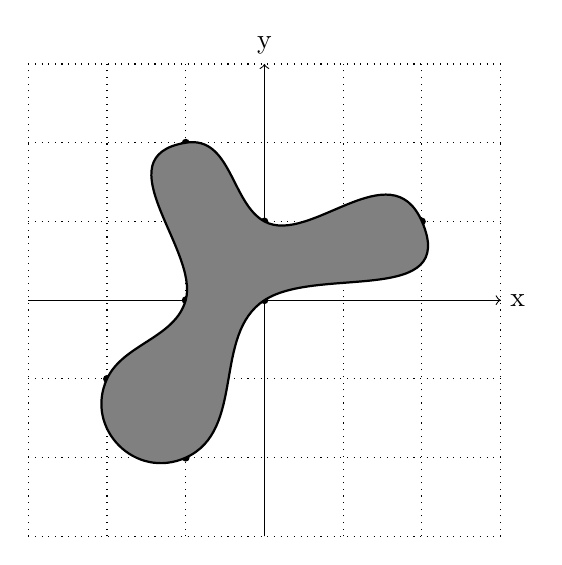
\begin{tikzpicture}
  \draw[step=1,thin,dotted] (-3,-3) grid (3,3);
  \draw[->] (-3,0) -- (3,0) node[right] {x};
  \draw[->] (0,-3) -- (0,3) node[above] {y};
  \foreach \c in {(0,0),(-1,-2),(-2,-1),(-1,0),
    (-1,2),(0,1),(2,1)} \fill \c circle (0.5mm);
  \draw[thick, fill=gray] (0,0) to[closed, curve through =
    { (-1,-2) (-2,-1) (-1,0) (-1,2) (0,1) }] (2,1);
\end{tikzpicture}
\end{document}
